\subsection{First definitions}

Nous commencerons dans cette section par donner quelques définitions pour introduire la théorie des espaces de Teichmuller.

\begin{dfnt}{Espace de Teichmuller}
Soit $S$ une surface de genre $g$, un marquage de $S$ est un couple $(X,f)$ formé d'une surface de Riemann $X$ et d'un homéomorphisme préservant l'orientaion $f:S \to X$.
Sur l'ensemble des marquages de $S$, nous pouvons faire une relation d'équivalence $(X_1,f_1) \sim (X_2,f_2)$ si il existe $\alpha : X_1 \to X_2 $ tel que $f_2 \circ \alpha \circ f_1^{-1}$ soit un homéomorphisme de $S$ préservant l'orientation et isotope à l'identité.
L'espace des marquages quotienté par la relation s'appelle l'espace de Teichmuller et est noté $\mathcal{T}_g$
\end{dfnt}

\begin{rmq}
Si $g \geq 2$, pour toute courbe simple fermée $\alpha$ de $S$, il existe une unique géodésique fermée de $X$ librement isotope à $f(\alpha)$. Nous noterrons $L_{\alpha}(X)$ sa longeur hyperbolique et nous prenons la topologie la plus faible sur $T_g$ qui rendent ces fonctions continues.
\end{rmq}

\begin{dfnt}{Espace des modules}
On appele groupe modulaire le groupe des homéomorphisme préservant l'oriention de $S$ quotienté par ceux isotope à l'identité.Nous notterons ce groupe $Mod_g$.
Il agit de façon discrète sur $T_g$ et l'espace quotient est appelé espace des modules et est noté $\mathcal{M}_g$
\end{dfnt}

Il est naturel de ce demander à quoi ressemble ces espaces.

\begin{dfnt}{Dehn twist}
Soit $\gamma$ une courbe simple et fermée. Il existe un voisinage tubulaire de $\gamma$ noté $A$ homéomorphe à $[0;1] \times S^{1}$.
On définit le Dehn's twist comme l'homéomorphisme qui vaut l'indentité hors de $A$ et vaut $(t,s) \mapsto (t,e^{2i \pi t} s)$ sur $A$.
\end{dfnt}

\begin{center}
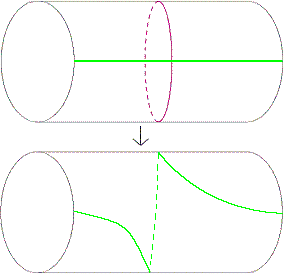
\includegraphics[width=6cm]{Image/Dehn_twist.png}
\end{center}

\begin{rmq}
Le théorème de Lickorisk affirme que le groupe modulaire est engendré par ces Dehn's twist et que plus précisément on peut choisir $2g+1$ générateurs \cite{Lickorish1964AFS}.
\end{rmq}

\begin{dfnt}{Measured foliation}
Given a surface $S$ and a finite set of points $P=(p_1,p_2,...)$, given a open covering $U_i$ on $S-P$, a collection of $C^1$
 real function $\nu_i$ such than $\| d \nu_j \| = \| d \nu_i \|$  on $U_i \cap U_j$,
 and near each singular point $p_s$ a coordinate neighborhood $V$ with complex coordinate $z$ such that $\| d \nu \| = \| Im(z^{\frac{k}{2}}dz) \|$ for some positive integer $k$ called the degree of the singular point,
 leaves of the foliations are the graphs immersed $S$ in along $dv$ is constant. In addition if each boundary circle pf $S$ is contained in a singular leaf, then ti is called a measurd foliation.
\end{dfnt}

The height $h_\gamma(\| d \nu \|)$ of a (free homotopy class) of a loop $\gamma$ on $S$ is the infinimum in the homotopy class of the integral by $\| d \nu \|$
\[
h_\gamma(\| d \nu \|)=inf_{\gamma \equiv \gamma'} \int_gamma \| d \nu \|
\]

The topology on the measured lamination that we will use is the weakest that make the height functions continous.

\begin{rmq}
We won't actually study the set of measured lamination but the equivalence class of \[
h_\gamma(\| d \nu \|)=h_\gamma(\| d \mu \|), \text{ for each loop} \gamma \in S
\].
We can equivalently use Whitehead equivalence relation on singular foliations by collapsing critical intervals to points and taking isotopy of foliation.
\end{rmq}

Let $\mathcal{MF}(S)$ be the space of all equivalence classes of measured foliations.
%TODO dessin et référence
\begin{dfnt}{Lamination}
Une lamination est un ensemble fermé qui est un union (non nécessairement finie) de géodésiques.
Par chaque point x contenu dans $\lambda$ il ne passe que une seul géodésique.
Nous notterons cet espace $\mathcal{ML}(x)$
\end{dfnt}

\begin{dfnt}{Geodesic currents}
Let $\mathcal{M}_\infty$ be the space of unordered pairs of distinct points in $\mathbb{S}^1$ \[
\mathcal{M}_\infty := {(z,w) \in \mathbb{S}^1 \times \mathbb{S}^1 , z \neq w}//(z,w) \equiv (w,z)
\]
Let $G$ be a discret torsion-free group in $PSL(2,\mathbb{R})$ such that $\mathbb{H}//G=S$ is a hyperbolic surface.
A geodesic current $\mu$ on $S$ is a $G$-invariant Radon measure on $\mathcal{M}_\infty$.
We will note $\mathcal{GC}(S)$ the space of geodesic currents.
\end{dfnt}

\begin{rmq}
$\mathcal{GC}(S)$ have a natural topology which is the weak $*$ convergence on continous functions.
\end{rmq}

\begin{rmq}
A mullticurve is a formel sum of geodesics $\gamma = \sum a_i \gamma_i$. The space of lamination is in some aspect the closure of the set of all multicurve
\end{rmq}

\begin{dfnt}{Intersection number}
Consider the square $\mathcal{M}_\infty^2 := \mathcal{M}_\infty \times \mathcal{M}_\infty $. In this space we can consider the open subset $\mathcal{IM}^2_\infty$ corresponding to pair pairs of geodesics which have transversal intersections in $\mathbb{H}$. G act on $\mathcal{IM}^2_\infty$.
If $\mu$ and $\nu$ are geodesic currents in $\mathcal{GC}(S)$, the product $\mu \times \nu$ define a $G$-invariant measure on $\mathcal{IM}^2_\infty$.
Finally if we take the mass of the total space $\mathcal{IM}^2_\infty // G$, the reasult is called the intersection number, $i(\mu,\nu)$
\end{dfnt}

\begin{prop}
\[
i: \mathcal{GC}(S) \times \mathcal{GC}(S) \to \mathbb{R}_+
\]
is continuous and bilinear
\end{prop}

\begin{rmq}
If $\alpha$ and $\beta$ are simple closed geodesics (dirac measure in $\mathcal{GC}(S)$), then the intersection number is the number of intersection between $\alpha$ and $\beta$.
Actually, one can define intersection in this way, first on simple closed geodesic, then by bilinearity on multi-curves and finally by continuity on geodesic current.
\end{rmq}

\begin{rmq}
The topology on $\mathcal{ML}$ is the weakest that make $i(.,.)$ a continous function.
\end{rmq}

\begin{dfnt}{Différentielle quadratique}
Une différentielle quadratique est une section du carré de l'espace tangeant canonique à X. Il s'écrit localement comme $\phi= \phi(z) dz^2$
\end{dfnt}

\begin{rmq}
Si $\phi(p) \neq 0$ on peut trouver une carte contenant $p$ dans laquel $\phi = dz^2$.
Ainsi $\phi$ détermine une métrique plate sur $X$ et un feuilletage $\mathcal{F}$ correspondant aux lignes horizontales.
\end{rmq}

Une différentielle quadratique est dite intégrable si \[
 \| \phi \| = \int_X | \phi | < \infty
\]
Nous notterons $\mathcal{Q}(x)$ l'espace de Banach des différentielles quadratiques intégrables.

\subsection{Flow on Teichmüller space}

We will define the main object of this paper, earthquake flow.

\begin{dfnt}
The earthquake flow is family of maps defined for $t \in \mathbb{R}$
\[
\begin{array}{crcl}

E_t: & \mathcal{ML}\times \mathcal{T}_g & \to & \mathcal{ML}\times \mathcal{T}_g \\

& (\lambda,X) & \mapsto & (\lambda,E_{t\lambda}X)

\end{array}
\]
where $E_\lambda$ is first defined on multi-curves $\gamma =\sum c_i \gamma_i$ by adding $c_i$ to the twist coordinate of $\gamma_i$.
As multi-curves are dense in lamination, we can show that it could be extend to the whole set $\mathcal{ML}$
\end{dfnt}

Thurston show that given two point in the Teichmüller space, there is a lamination $\lambda$ such that the earthquake flow from one point with respect to $\lambda$ reach the other point.

We can ask ourselves what is an invariant measure of this flow.

\begin{dfnt}
The Weil-Peterson form is the the form \[
\omega_{WP} = \sum d l_i \wedge d \tau_i
\]
Where $(l_1,...,\tau_1)$ are the Fenchel-Nielsen according to a pant decomposition.

This give a measure $\mu_{WP}$.
\end{dfnt}

There is a finite measure $\nu_g$ in the Lebesgue measure class on $\mathcal{P}^1 \mathcal{M}_g$ which is invariant under the earthquake flow. This measure projects to the volume form given by $B(X) \times \mu_{WP}$ on $\mathcal{M}_g$, where \[
B(X)=\mu_{Th}(\lambda \in \mathcal{ML}, l_\lambda(X) \leq 1)
\]

There are two other important flows, the geodesic flow and the horocyclic flow.
First there is a natural homeomorphism between $T^1 \mathbb{H}  \simeq PSL_2(\mathbb{R})$, since $PSL_2(\mathbb{R})$ act simply trasnsitively on it. This morphism can be choosen up to a conjugaison via an other element of $PSL_2(\mathbb{R})$. We we will be interested in a special kind of subgroup.

\begin{dfnt}
A fuchsian group $\Gamma$ is a finitely generated and discrete subgroup of $PSL_2(\mathbb{R})$. Then $\Gamma$ act discontinuously on $\mathbb{H}$.
\end{dfnt}

Then a Hyperbolic surface can be represented as $PSL_2(\mathbb{R})/ \Gamma$. If $U$ is a one parameter subgroup of $PSL_2{\mathbb{R}}$ it act on the quotient.

There are two important exemple:

\begin{dfnt}
The geodesic flow is a flow on the Teichmuller space given by the action of the diagonal matrices\[
u_t=\begin{pmatrix}
e^t & 0 \\
0 & e^{-t}
\end{pmatrix}
\]
\end{dfnt}

\begin{dfnt}
The horocycle flow is a flow on the bundle of nonzero quadratic differential, $\mathcal{QD}$, of the Teichmuller space given by the unipotent action of \[
u_t=\begin{pmatrix}
1 & t \\
0 & 1
\end{pmatrix}
\]
\end{dfnt}

The geodesic flow is also the flow that we obtain by following geodesic line on $\mathbb{H}$ and the horocycle is the flow we obtain by following curves which are everywhere orthogonal to the geodesic, which is the horizotal line and the circle tangent to the real line.

\begin{figure}[h!]
\centering
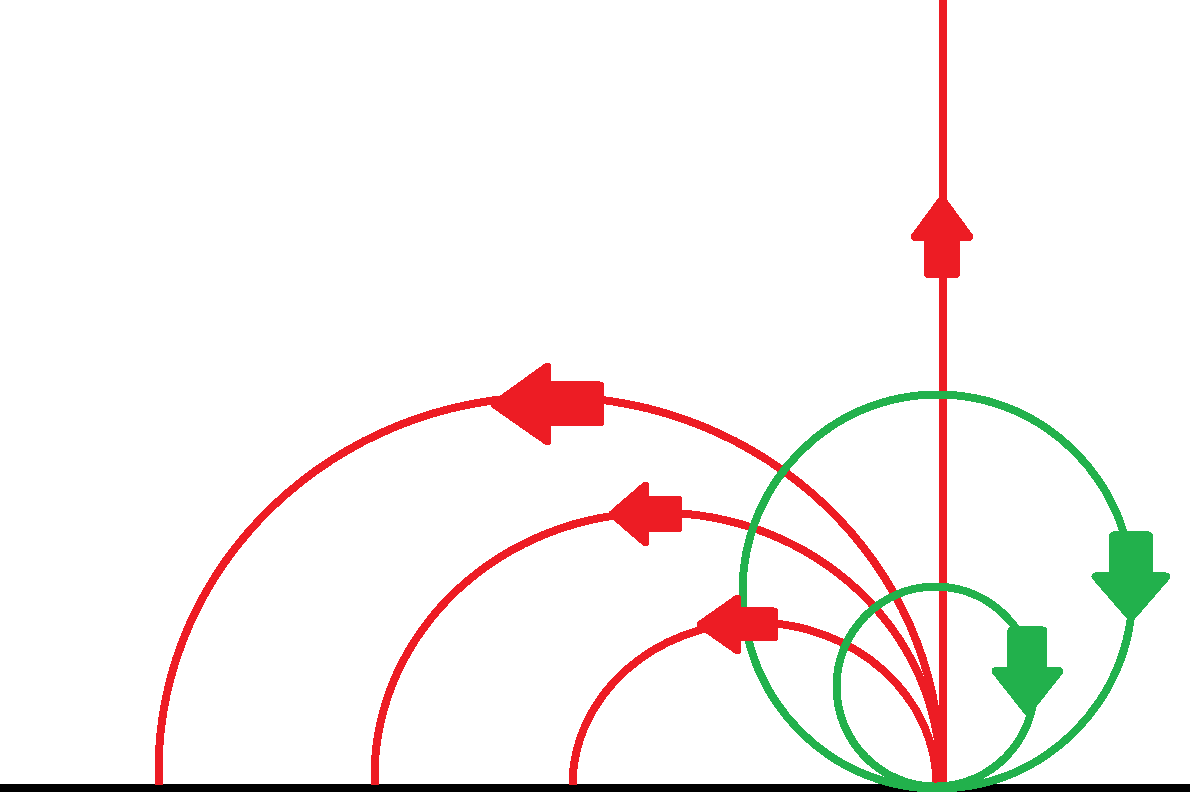
\includegraphics[width=6cm]{Image/FlowPaint.png}
\caption{Representation of the horocycle flow, in green, and the geodesic flow, in red}
\end{figure}


An important relation is how this two flows interact between each other \[
\begin{pmatrix} e^t & 0 \\ 0 & e^{-t}\end{pmatrix} u_t=\begin{pmatrix} 1 & s \\ 0 & 1 \end{pmatrix} \begin{pmatrix} e^{-t} & 0 \\ 0 & e^{t}\end{pmatrix}=
\begin{pmatrix} 1 & s e^{2t} \\ 0 & 1\end{pmatrix}
\]
So the the conjugaison of the horocyclic flow by the geodesic one is still the horocyclic flow.

\begin{figure}[h!]
\centering
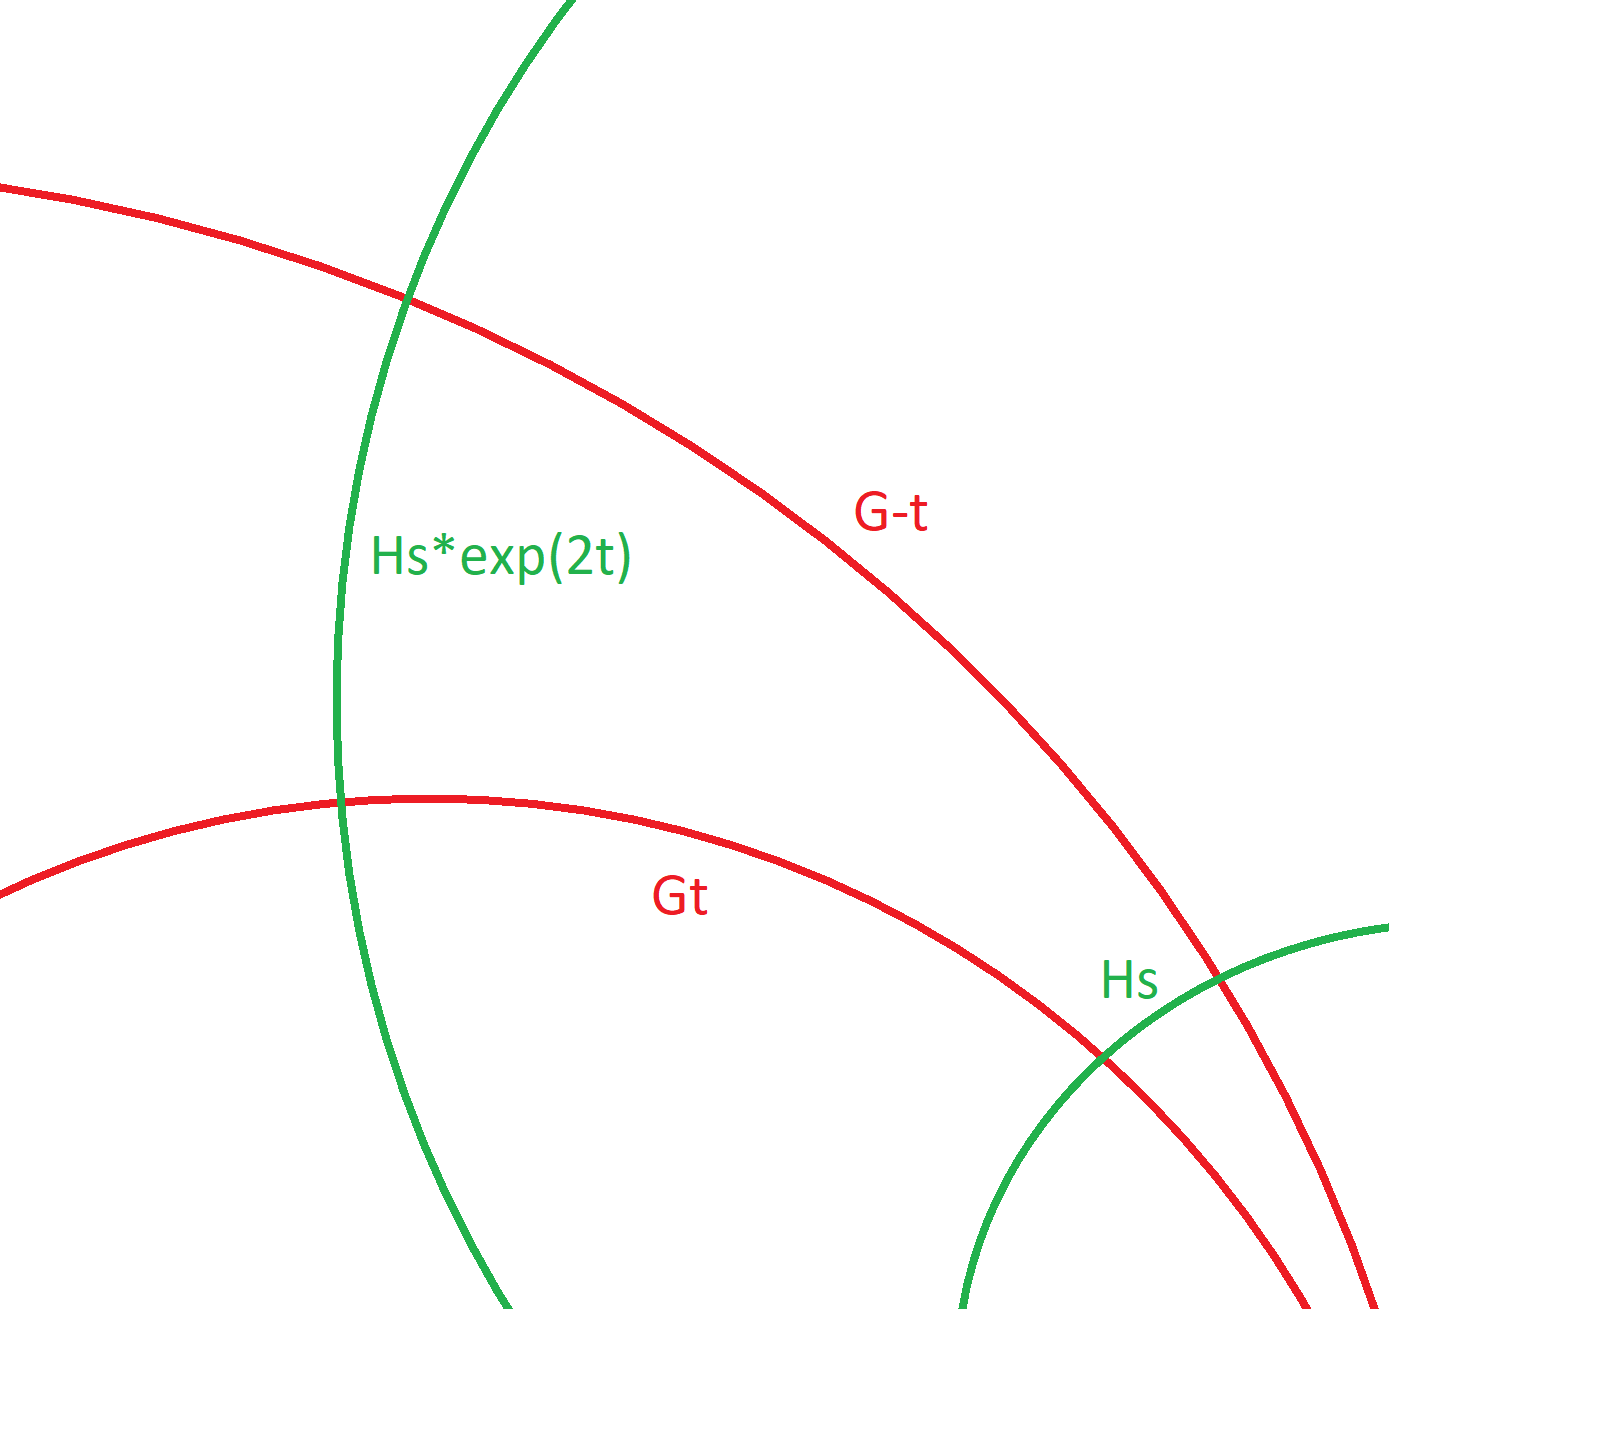
\includegraphics[width=6cm]{Image/Commutatoin.png}
\caption{The conjugaison of the horocycle flow by the geodesic one.}
\end{figure}

%TODO faire l'exercice du pdf sur les flots.

\subsection{Decomposition of hyperbolic surface}

One way to construct all hyperbolic surface is to decompose them in elementary piece, that we will call pair of pant.

A hyperbolic geometric exercice show that a hexagone which side are geodesics and with right angles is determined by the lenght of three sides which are not consecutifs.
%TODO Faire cette exercice

\begin{center}
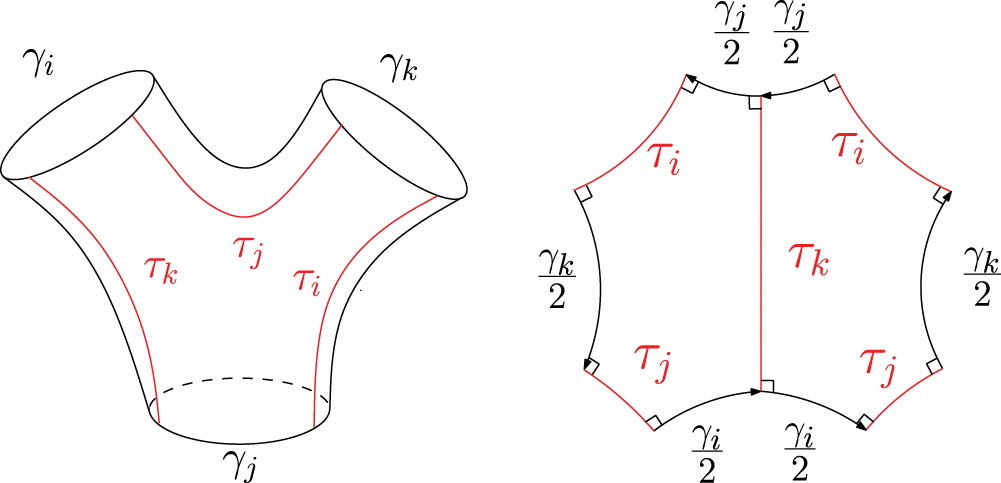
\includegraphics[width=12cm]{Image/PairOfPant.jpg}
\end{center}

 On the image above $\gamma_i$, $\gamma_j$ and $\gamma_k$ determined the hexagone. Then we can glued them to have a pair of pant.

 \begin{dfnt}
 A pair of pant is a hyperbolic surface with three geodesic boundaries and no ponctured.
 \end{dfnt}

\begin{rmq}
The pair of pant is uniquely determined by the lenght of the three boundarie geodesics.
\end{rmq}

\begin{rmq}
The lenght of one or more geodesic can go to zero and the boundaries become a ponctured.
\end{rmq}

We can now decompose, with the following theorem, all hyperbolic surfaces in a collection of pair of pants.

\begin{thm}
Let $S$ be a surface of genus $g$ and with $n$ ponctured. There is a set of $3g-3+n$ simple closed curves $(\gamma_1,...,\gamma_{3g-3+n})$ such that $S\ \Cup \gamma_i$ is a disjoint collection of pair of pants.
\end{thm}

\begin{dfnt}
Given a surface $S$ and a pant decomposition $\gamma_1,...,\gamma_{3g-3+n}$, we have a map \[
\mathcal(S) \rightarrow (\mathbb{R^{+}}^{3g-3+n},\mathbb{R}^{3g-3+n}) \\
X \mapsto (l_{\gamma_1}(X),...,l_{\gamma_{3g-3+n}}(X),\tau_{\gamma_1}(X),...,\tau_{\gamma_{3g-3+n}}(X))
\]
This map is injective and is call the Fenchel-Nielsen cordinates.
\end{dfnt}

\subsection{The collaring theorem}

We will give a lemma which is useful to determine if the minimal length of a geodesic crossing an other one.

We define the function \[
\eta(l)= \frac{1}{2} ln(\frac{cosh(l/2)+1}{cosh(l/2)-1})
\]

\begin{dfnt}
Let $\gamma$ be a simple closed geodesic of length $l$ on a hyperbolic surface $X$. If the $\delta$-neighborhood \[
A_\delta(\gamma):= \{ x \in X | d(x,\gamma) < \delta \}
\]
is isometric to the $\delta$-neighbohood of the unique simple closed geodesic on the cylinder of modulus $\frac{\pi}{l}$, we say that $\gamma$ admit a $\delta$-collar
, or that $A_\delta(\gamma)$ is the $\delta$-collar of $\gamma$.
\end{dfnt}

Then we have

\begin{thm}
Let $X$ be a complete hyperbolic surface, and let $\Gamma:={\gamma_1,...}$ be a collection of disjoint simple closed geodesic, each $\gamma_i$ of length $l_i$. Then $A_{\eta(l_i)}(\gamma_i)$ are collars around the $\gamma_i$, and they are disjoint.
\end{thm}

\begin{cor}
Let $X$ be a hyperbolic surface, and $\gamma_1$, $\gamma_2$ two simple closed geodesics on $X$ of lengths $l_1$ and $l_2$. If $l_1 < 2 \eta(l_2)$, then either $\gamma_1=\gamma_2$ or $\gamma \cap \gamma_2 = \emptyset$
\end{cor}

\begin{cor}
Let $X$ be a hyperbolic surface, and let $\gamma_1$, $\gamma_2$ be two simple closed geodesics with lengths $< ln(3+2 \sqrt{2})$. Then either $\gamma_1=\gamma_2$ or $\gamma_1 \cap \gamma_2 = \emptyset$.
\end{cor}

%TODO Mettre des figures et des démonstrations
